\documentclass[smallcondensed]{svjour3}     % onecolumn (ditto)
\usepackage[misc]{ifsym}
\smartqed  % flush right qed marks, e.g. at end of proof
%
\usepackage{graphicx}

\journalname{Information Science}

\usepackage{epsfig}
\usepackage{epstopdf}
\usepackage{url,overcite}
\usepackage{algorithm}
\usepackage{algorithmicx}
\usepackage[noend]{algpseudocode}
\usepackage{subfigure}
\usepackage[colorlinks,linkcolor=blue,citecolor=blue,anchorcolor=black,urlcolor=blue]{hyperref}
\usepackage[doipre={DOI:}]{uri}
\usepackage{booktabs}
\usepackage{threeparttable}
\usepackage{graphicx}
\usepackage{epsfig}
\usepackage{mathtools}
\usepackage{multirow}
\usepackage{float}
\usepackage{longtable}
\usepackage{enumerate}
\usepackage{bm}
\usepackage{xcolor}

\usepackage[all]{hypcap}

\usepackage[numbers]{natbib}
\usepackage{amsfonts}

\begin{document}

\title{Enhanced path planning through GAN Predictions}

\author{Kun He and Fan Min*\thanks{Corresponding author. E-mail: minfan@swpu.edu.cn (Fan Min).} }

\institute{
Kun He\\
School of Computer Science, Southwest Petroleum University, Chengdu 610500, PR China\\
\email{hk20201008@163.com}\\
\\
Fan Min\\
School of Computer Science, Southwest Petroleum University, Chengdu 610500, PR China\\
\email{minfan@swpu.edu.cn}
}
\date{Received: date / Accepted: date}
% The correct dates will be entered by the editor

\maketitle

\begin{abstract}
Path planning is a crucial task in robotics.
Sampling-based algorithms have garnered significant attention for this purpose. 
However, traditional sampling-based algorithms suffer from poor initial path quality and low efficiency. 
In this paper, we present a new learning-based path planning method. 
First, we utilize a generative adversarial network to learn from previous successful planning experiences
Second, use it to restrict the sampling area in a new map. 
We then employ RRT* to generate a better initial path by performing path planning within this restricted area. 
We propose a total of 20 maps, each with varying complexities. 
Out of these, 16 are used for training and testing, while the remaining 4 are used to test the proposed method's generalization ability. 
We compare our approach with three state-of-the-art methods.
The results demonstrate that our method outperforms them in both path quality and convergence speed.
\keywords{Sampling-based path planning \and Optimal path planning \and GANs}
\end{abstract}

\section{Introduction}\label{sec:introduction}
Robot path planning refers to finding a safe and feasible path for the robot in a given map state space, so that the robot can reach the target position from the starting point. 
According to the nature of the method, common robot path planning algorithms can be divided into the following categories:

Grid-based path planning algorithms: These algorithms usually divide the map into a grid graph, and then use the shortest path search algorithm to find the optimal path. 
For example Dijkstra's algorithm \cite{dijkstra1959note}, A* \cite{hart1968formal}, D* algorithms. 
This type of method transforms the path planning problem into a path search problem in the graph, and the efficiency of this type of algorithm is related to the path quality and the resolution of the grid division.

Bionic-based path planning algorithms: These algorithms typically use biological information to explore maps to guide robot path planning. 
Such as genetic algorithm, particle swarm algorithm, ant colony algorithm. 
These algorithms are simple to implement, but require multiple iterations to obtain suboptimal paths, and are prone to getting stuck in local minima.

Sampling-based path planning algorithms: These algorithms usually use random sampling to explore the map, use a tree or graph to store path information, and then use the shortest path search to get the final path. 
For example Rapidly Exploring Random Tree (RRT) \cite{lavalle2001rapidly}, Rapidly Exploring Random Tree-star (RRT*) \cite{karaman2011sampling}, Probabilistic Roadmap (PRM) \cite{kuffner2000randomized}. 
This type of algorithm is fast, but it is usually difficult to obtain the optimal path.

Rapidly Exploring Random Tree (RRT) is a popular algorithm in robot path planning. 
RRT is a very effective path planning algorithm that can cope with various complex environments. 
And it is easy to extend to high-dimensional space and add dynamic constraints, and more importantly, it guarantees probabilistic completeness.
However, the quality of the initial paths obtained by RRT is poor because it is prone to unnecessarily long paths or zigzag paths. 
To address this issue, researchers have developed several variants of the RRT algorithm, such as RRT*. 
It is an improvement over the basic RRT algorithm. 
RRT* adds neighbor search and rerouting to ensure asymptotically optimal path quality. 
In short, RRT* optimizes the existing paths while exploring the space, thus ensuring asymptotic optimality. 
But to obtain high-quality paths means more iterations are needed, which means that RRT* cannot achieve a balance between path quality and efficiency.

To alleviate this shortcoming, we propose a path planning method based on Generative Adversarial Networks.
Our algorithm speeds up path planning by constraining the search space. 
First, our model is trained using successful planning experience to obtain a path planner. 
Subsequently, the restricted sampling area is predicted using the trained planner. 
Finally, a sampling-based approach is used to sample over the region. 
The restricted sampling area can avoid RRT* blind search, thus speeding up the sampling process and obtaining better initial paths.

Our contributions are summarized as follows:
\begin{enumerate}[1)]
	\item A new path planning method is proposed.
	\item A new path planner is proposed.
	\item A new path planning dataset is proposed and the feasibility of our scheme is verified.
\end{enumerate}

\section{Related work}\label{section: related-work}
Over the past few years, there have been many research efforts devoted to improving the performance of the underlying RRT algorithms.

Changing the iteration method or sampling strategy of RRT is a feasible way.
RRT-connect \cite{kuffner2000rrt} proposes a new way to iterate tree nodes bidirectionally.
It takes the starting point and the ending point as the root nodes of the two trees respectively, and iteratively explores the state space alternately until the two trees meet.
The efficiency of RRT-connect to explore the state space has been significantly improved, but the paths it generates still need to be optimized.
Informed-RRT* (IRRT*) \cite{2014irrt} uses the same iteration and optimization strategy as RRT*.
However, IRRT* builds an ellipse with the start and end points as foci, and performs a heuristic search within the ellipse, which makes IRRT* converge faster.
KB-RRT* \cite{WANG2021114541} is a random tree algorithm for bidirectional exploration, which introduces pruning operations in the iterative process to make the final path better.

Using known information to search can improve the quality of generated paths.
P-RRT* constructs the gravitational repulsion field through the state space, so as to obtain a more efficient convergence speed.
GMR-RRT* learns from past successes, resulting in faster convergence and path quality in known environments.
However, GMR-RRT* may perform poorly in unfamiliar environments.

Using deep learning models to improve the performance of RRT is a promising direction.
N-RRT* \cite{2020Neural} is the most reliable path planning algorithm based on convolutional neural network.
It uses the CNN model to learn a large number of successful path planning cases generated by A*, and uses the learned model to predict the probability distribution of the optimal path of the new map.
It is then used to guide the sampling process, resulting in good quality paths.
CGAN-RRT* uses pix2pix as the generator structure of GAN \cite{NIPS2014_5ca3e9b1} to predict the better exploration area of the map, thereby speeding up the sampling process of RRT*, with better efficiency and better path quality.
LM-RRT is a novel learning-based multi-RRT method for robot path planning in narrow passages.
It guides multiple RRTs to explore the state space through reinforcement learning, and this strategy can enhance the exploration ability of RRTs.
However, the exploration process may consume a lot of resources.

\section{Preliminaries}\label{section: Preliminaries}
In this section, we briefly introduce the related concepts of path planning, the Markov clustering algorithm, and RRT*.

\subsection{Path Planning Problem}\label{subsection: path planning problem}
The data model of the path planning problem can be represented by a 5-tuple:
\begin{equation}\label{equation: model}
(\bm{\chi}, \bm{\chi}_{\textrm{obs}}, x_{\textrm{sou}}, x_{\textrm{tar}}, r),
\end{equation}
where
\begin{enumerate}[1)]
	\item $\bm{\chi} \subset \mathbb{R}^n$ is the \emph{state space}, usually $n \in \{2, 3\}$;
	\item $\bm{\chi}_{\textrm{obs}} \subset \bm{\chi}$ is the \emph{obstacle state space};
	\item $x_{\textrm{sou}} \in \bm{\chi} \setminus \bm{\chi}_{\textrm{obs}}$ is the \emph{source};
	\item $x_{\textrm{tar}} \in \bm{\chi} \setminus \bm{\chi}_{\textrm{obs}}$ is the \emph{target};
	\item $r$ is the radius of the \emph{target}.
\end{enumerate}

Moreover, $\bm{\chi}_{\textrm{fre}} = \bm{\chi} \setminus \bm{\chi}_{\textrm{obs}}$ is the \emph{obstacle-free state space}.
Let $\bm{\chi}_{\textrm{tar}} = \{x \in \bm{\chi}_{\textrm{fre}} \vert \lVert x - x_{\textrm{tar}} \rVert < r\}$ be the \emph{target} space.
The path planning problem is to find an \emph{obstacle-free feasible continuous path} $\bm{\sigma} \subset \bm{\chi}_{\textrm{fre}}$ from $x_{\textrm{sou}}$ to any $x \in \bm{\chi}_{\textrm{tar}}$.
That is, we only need to reach the neighborhood of $x_{\textrm{tar}}$.
The path is defined as a sequence
\begin{equation}\label{equation: path}
	\bm{\sigma} = \sigma_0 \sigma_1 \dots \sigma_m,
\end{equation}
where $\sigma_0 = x_{\textrm{sou}}$, $\sigma_m \in \bm{\chi}_{\textrm{tar}}$,
$\forall \lambda \in [0, 1], \lambda \sigma_i + (1 - \lambda)\sigma_{i - 1} \in \bm{\chi}_{\textrm{fre}} (i = 1, 2, \dots, m)$, and
	the direct connection between $\sigma_i$ and $\sigma_{i - 1}$ is obstacle-free.
In other words, the path is essentially a polyline in the map.

The cost of the path is defined as the length of the polyline, i.e.,
\begin{equation}\label{equation: path-cost}
	c(\bm{\sigma}) = \sum_{i=1}^{m} \lVert \sigma_i - \sigma_{i - 1} \rVert,
\end{equation}
where $\lVert \cdot \rVert$ is the $l_2$ norm of a vector.

The path planning problem is to find an optimal path
\begin{equation}\label{equation: optimal-path}
	\bm{\sigma}^* = \mathop{\arg\min} \limits_{\bm{\sigma}} c(\bm{\sigma}).
\end{equation}

\subsection{GAN}
GAN consists of two components: a generator and a discriminator.
The generator generates an image $G_\theta (z)$ using noise $\textbf{z}$ from the noise space $\textbf{z} \in \mathbb{R}^n $.
The discriminator generates an image $G_\theta (z)$ using data $\textbf{x}$ from data space $\textbf{x} \in \textbf{X}$.

The generator and discriminator can be thought of as playing a game:
The generator is trained to generate samples that are as realistic as possible, while the discriminator is trained to correctly classify samples as real or fake.
The generator and discriminator networks are trained alternately, with the generator network trying to fool the discriminator, and the discriminator network trying to classify the samples correctly.

The objective function of Gan can be expressed as:

\begin{equation}\label{equation: objective funtion-gan}
	\min_{\theta} \max_{\phi} ( \mathbb{E}_{\mathbf{x} \sim \textbf{p}_{\textrm{data}}}[\log D_\phi(\textbf{x})] + 
	\mathbb{E}_{\mathbf{z} \sim p(\textbf{z})}[\log (1-D_\phi(G_\theta(\textbf{z})))] )
\end{equation}

The loss function of Gan can be expressed as:



\subsection{RRT*}\label{subsection: rrt-star}
Among the sampling-based algorithms, RRT* is one of the representative algorithms that are widely used.
RRT* explores the \emph{state space} by expanding space-filling trees
\begin{equation}\label{equation: space-filling trees}
	T = (\mathbf{N}, r, p)
\end{equation}
where
\begin{enumerate}[1)]
	\item $\mathbf{N}$ is the set of all nodes in the tree;
	\item $r \in \mathbf{N}$ is the root node;
	\item $p: \mathbf{N} \to \mathbf{N} \cup \{\phi\}$ is the parent mapping satisfying
	\begin{enumerate}[a)]
		\item $p(r) = \phi$;
		\item $\forall n \in \mathbf{N}, \exists ! \ i \geq 0, \textrm{s.t. } p^{(i)}(n) =r$;
		\item $\phi$ represents the empty node.
	\end{enumerate}
\end{enumerate}

\section{The proposed algorithm}
In this section, we first describe the implementation of CGRRT.
Then, we prove the probabilistic completeness of CGRRT.

\subsection{network structure}


\begin{figure}
\centering
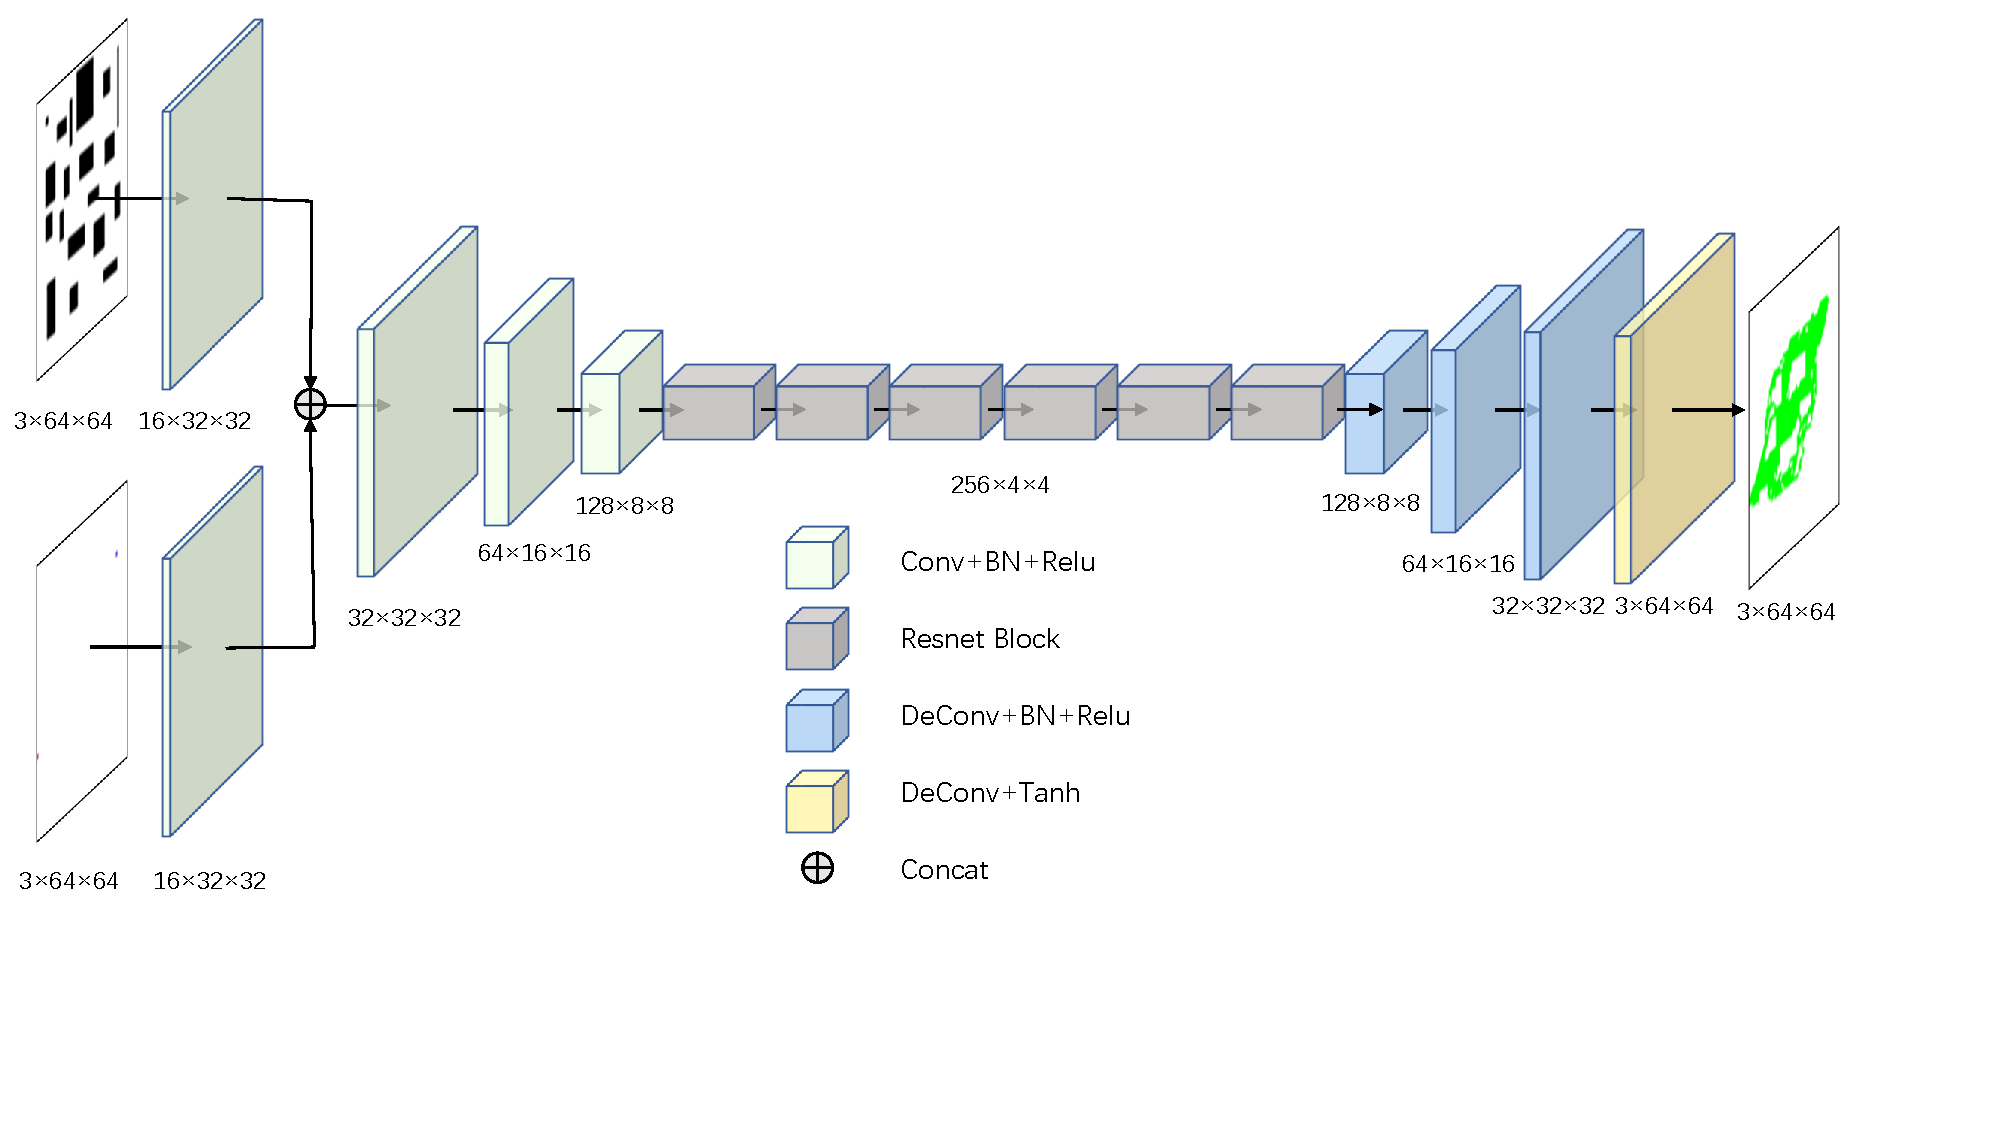
\includegraphics[scale=0.3]{network-generator.pdf}%%%%%%%%%%%%%%%%scale=缩小比例,或者用width=2in
\caption{generator}     
\label{fig:generator}
\end{figure}

\begin{figure}
\centering
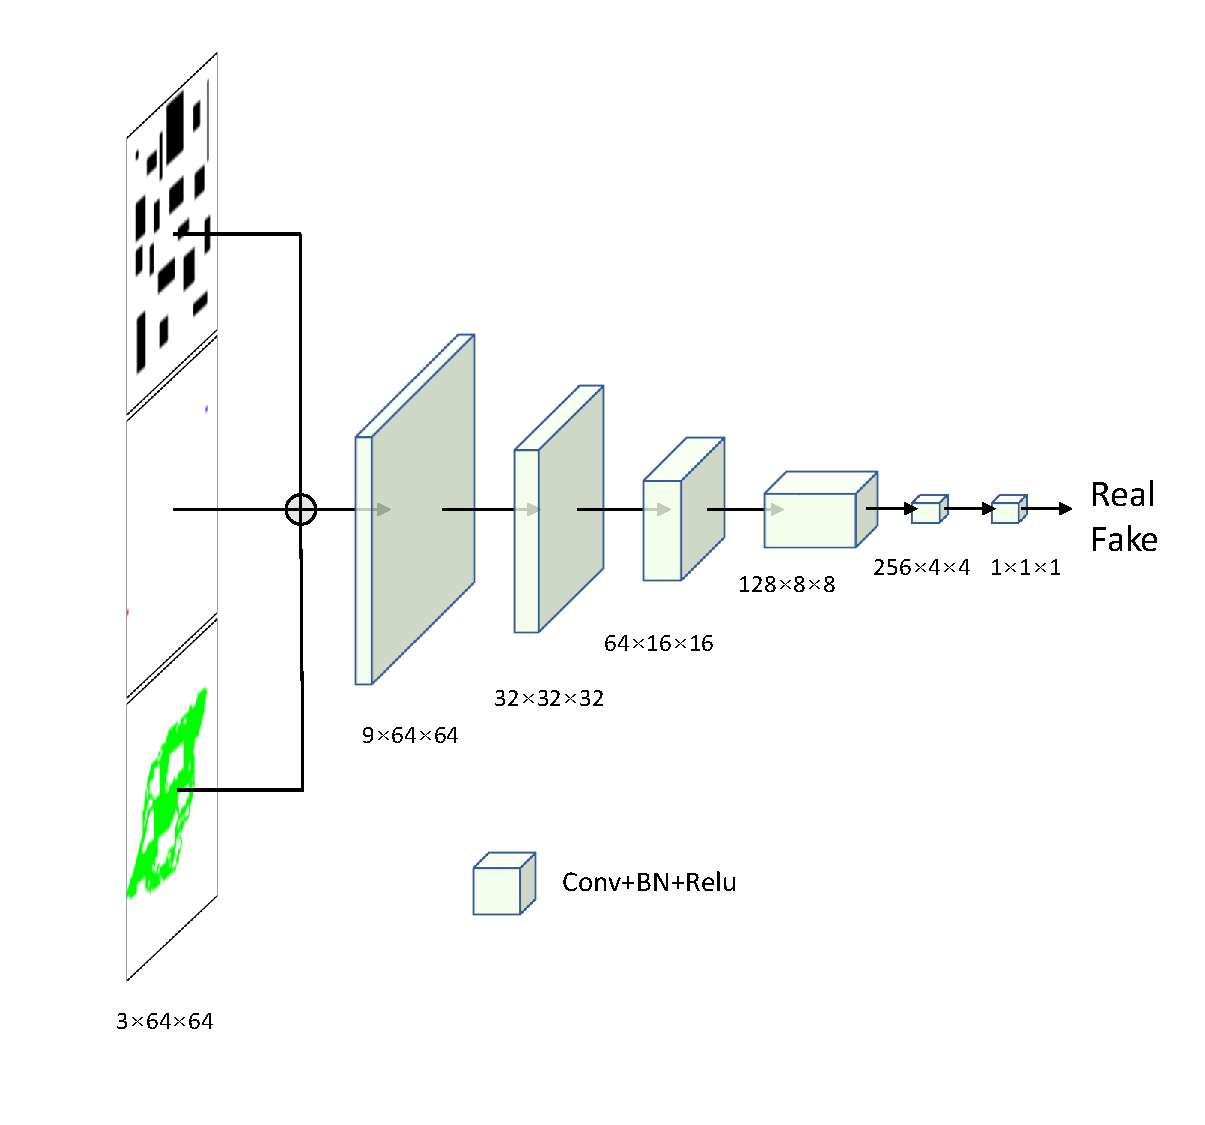
\includegraphics[scale=0.3]{network-discriminator.pdf}%%%%%%%%%%%%%%%%scale=缩小比例,或者用width=2in
\caption{discriminator}     
\label{fig:discriminator}
\end{figure}


\subsubsection{GAN}
Generative Adversarial Networks (GANs) are a class of deep learning models that have received a lot of attention in recent years due to their ability to generate high-quality synthetic images and other media. 

GAN consists of two neural networks: a generator network and a discriminator network. 
The generator network is trained to synthesize new data samples similar to a given training dataset, while the discriminator network is trained to distinguish real samples from fake samples.
The training process of GANs involves an adversarial game between the generator and discriminator networks. 
Specifically, the generator network is trained to generate samples that are as realistic as possible, while the discriminator network is trained to correctly classify samples as real or fake. 

The generator and discriminator networks are trained alternately, with the generator network trying to fool the discriminator, and the discriminator network trying to classify the samples correctly.
A key challenge in training GANs is balancing the performance of the generator and discriminator networks. 

If the generator network is too weak, it will not be able to synthesize real samples, and if the discriminator network is too weak, it will not be able to effectively distinguish real samples from fake samples. 
To solve this problem, GANs use specific objective and loss functions to guide the training process.
The objective function of GAN is usually defined as a min-max game, where the generator network tries to minimize the loss function, while the discriminator network tries to maximize the loss function.
The loss function is usually defined as binary cross-entropy loss, which measures the difference between the predicted label (true or fake) and the ground truth label.


\subsection{GAN-RRT*}
In this study, we feed the map as an RGB image into a trained CycleGan to predict regions with a high probability of success. 
The purpose is to mitigate the poor quality and inefficiency of the RRT* algorithm when it first finds a path. 
To achieve this, we use a GAN to learn areas of paths successfully planned by the RRT* algorithm in the past to predict promising areas in the new map.

After obtaining the predicted promising region, we use the RRT* algorithm for path planning in this region.
The RRT* algorithm is a path planning algorithm based on random trees, which can quickly find a reasonable path in a complex environment. 
In this study, we use the RRT* algorithm to quickly find plausible paths within predicted promising regions. 
Finally, we take the obtained path as the output of the proposed algorithm.

We hope that the method of this research can improve the efficiency and quality of robot path planning in complex environments.

\begin{algorithm}
	\caption{Enhanced RRT* with Clustering and Presearching (ERCP)}
	\label{algorithm: ercp-RRT*}
	\hspace*{0.02in} {\bf Input:} $\bm{\chi}, \bm{\chi}_{\textrm{obs}}, x_{\textrm{sou}}, x_{\textrm{tar}}, \bm{\chi}_{\textrm{opt}}, r$ \\
	\hspace*{0.02in} {\bf Output:} $T$
	\begin{algorithmic}[1]
		\State $\mathcal{M} \leftarrow Generator(\bm{\chi}, \bm{\chi}_{\textrm{obs}}, x_{\textrm{sou}}); $
		\State $T = (\mathbf{N}, r, p) \leftarrow (\emptyset, x_{\textrm{sou}}, \emptyset) ;$
		\State $\bm{\chi}_{\textrm{tar}} \leftarrow \{x \in \bm{\chi}_{\textrm{fre}} \vert \lVert x - x_{\textrm{tar}} \rVert < r\} ;$
		\For {$i \in \{1, 2, \dots, k\}$}
			\State $x_{\textrm{ran}} \leftarrow SampleFrom(\bm{\chi}_{\textrm{opt}}) ;$
			\State $x_{\textrm{nst}} \leftarrow Nearest(x_{\textrm{ran}}) ;$
			\State $x_{\textrm{new}} \leftarrow Steer(x_{\textrm{nst}}, x_{\textrm{ran}}) ;$

			\If {$obstacleFree(x_{\textrm{nst}}, x_{\textrm{new}})$}
				\State $\mathbf{N} \leftarrow \mathbf{N} \cup x_{\textrm{new}} ;$
				\State $p(x_{\textrm{new}}) = x_{\textrm{nst}} ;$
				\State $X_{\textrm{nea}} \leftarrow NearestNeighborSearch(T, r) ;$
				\State $T \leftarrow Rewiring(X_{\textrm{nea}}, x_{\textrm{new}}) ;$
				\If{$x_{\textrm{sou}} \in \bm{\chi}_{\textrm{tar}}$ }
					\State Return $T ;$
				\EndIf
			\EndIf
			%\EndIF
		\EndFor
		\State Return $failure ;$
	\end{algorithmic}
\end{algorithm}

\section{Experiments}\label{section: Experiments}
In terms of dataset, we use 20 initial maps and generate 200 different maps through data augmentation. 
Then for each map, randomly select 100 pairs of start and end points, use RRT to find feasible paths among them, 50 successful paths form the promising areas of the map, and finally generate 20,000 sets of data.

In terms of training, we use 16,000 sets of data as training tests, the ratio of training and testing is 4:1, and another 4,000 sets of untrained data are used to evaluate the generalization ability of the model.

In terms of evaluating model performance, we compare our model with the three most popular algorithms (RRT*, IRRT*, SaGan). 
Among them, IRRT* realizes the heuristic search of ellipse in the path planning process, which speeds up its convergence to the optimal solution. 
SaGan learns the features of maps and promising regions through residuals and attention, thus giving promising regions between different starting and ending points.

We use windows10 as the training and testing platform of the model, the CPU is AMD Ryzen-7 4800H, the graphics card is RTX 2060 6g, and the memory is 16g. 
In terms of software, the model implementation language is python3.8, and the deep learning framework is pytorch 1.12.1.

\subsection{Dataset}

\begin{figure}
\centering
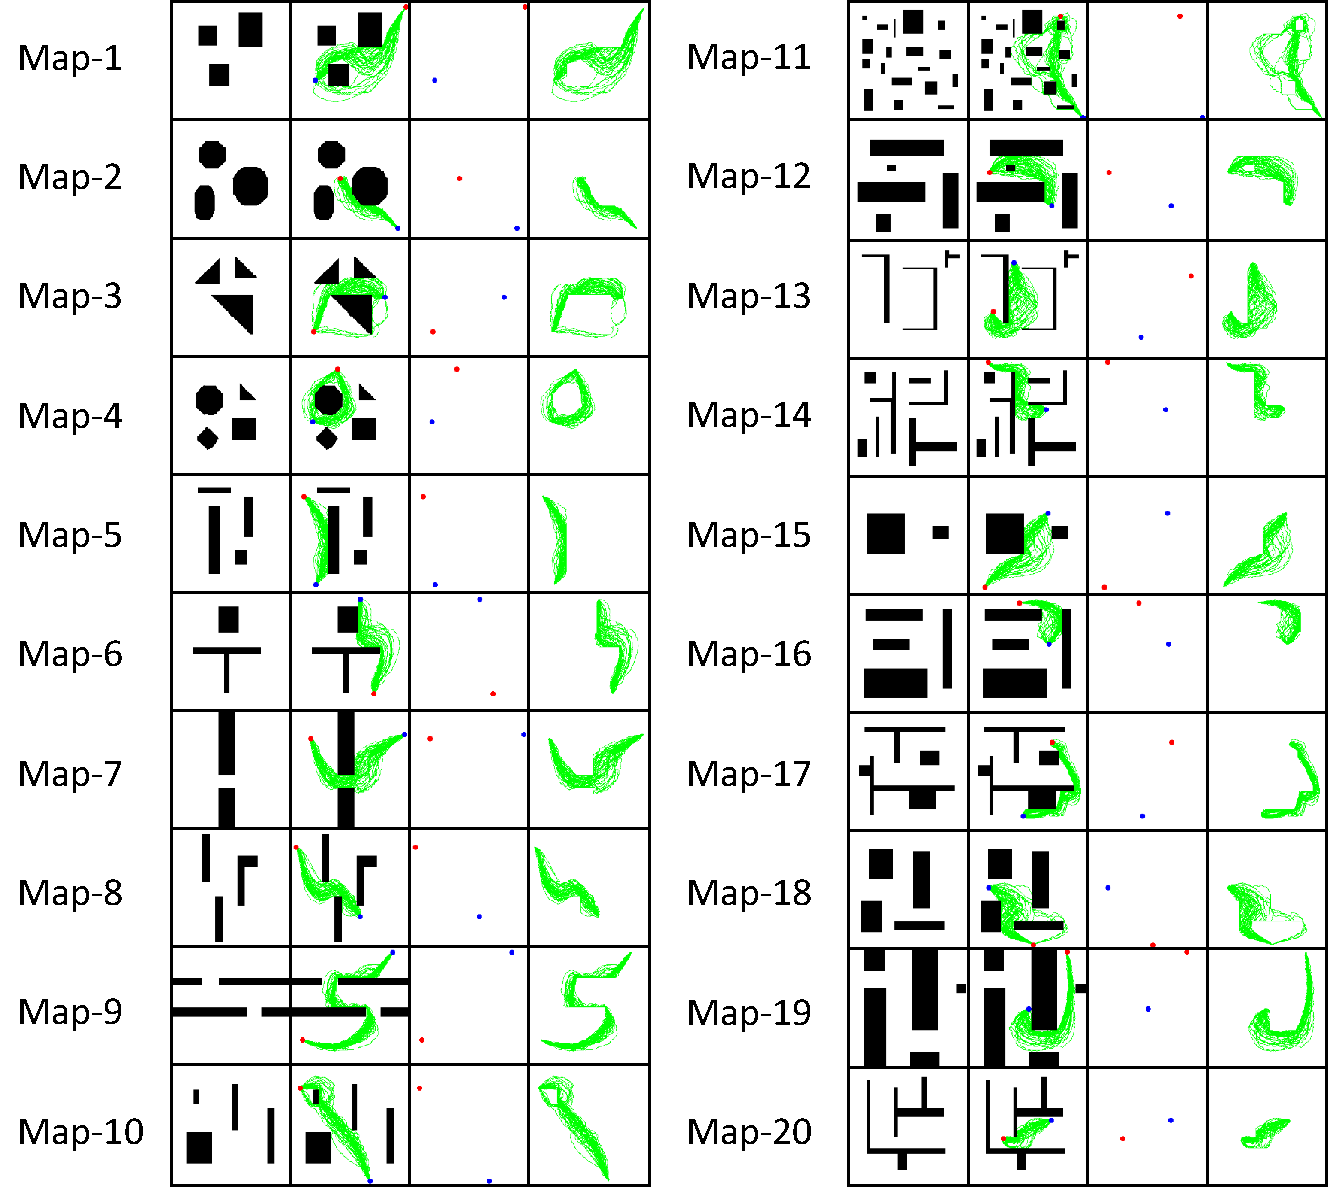
\includegraphics[width=1\linewidth]{data-set-256.pdf}
\caption{Display of the original dataset.
On the left is the map name.
The black parts are obstacles.
The blue dot is the starting point and the red dot is the end point.
The green area is ground truth.
The first column is the original map.
The second column is the data, including the start and end points, and ground truth.
The third column is the start and end of the separation.
The fourth column is the separated ground truth.
}     
\label{fig: data-set}
\end{figure}

We generated 20 maps of different complexity.
In order to enhance the generalization ability of the model, nine extended maps are generated by translating and rotating obstacles for each map.
The final map total is 200.

By randomly selecting the starting point and the ending point in the map, use RRT to perform 50 random iterations on this map. 
Then collect the paths that successfully connect the starting point and the ending point to form ground truth.

Partial data is shown in Fig. \ref{fig: data-set}, which shows one set of data for each map.
On the far left of the map is the name of the map.
The first column is a map with only obstacles, and the black parts are obstacles.
The second column contains obstacles, start and end points, and ground truth.
The blue dot is the starting point and the red dot is the end point.
The green area is ground truth.
The third column of pictures is the start and end points extracted separately on the left.
The pictures in the fourth column are promising regions.

The purpose of extracting the start point, end point, and desired area separately is to facilitate data processing.

\subsection{Evaluate model performance}
The connectivity of the generated promising regions is the key to evaluate the performance of our model, i.e. whether the promising regions can successfully connect the start and end points.
The evaluation method is to use the breadth-first traversal method, starting from the starting point, and only passing through the promising area to successfully reach the end point.

Our model is calculated to be 85.08\% connected in the trained map using the promising regions obtained from the test set.

\begin{figure}
	\centering
	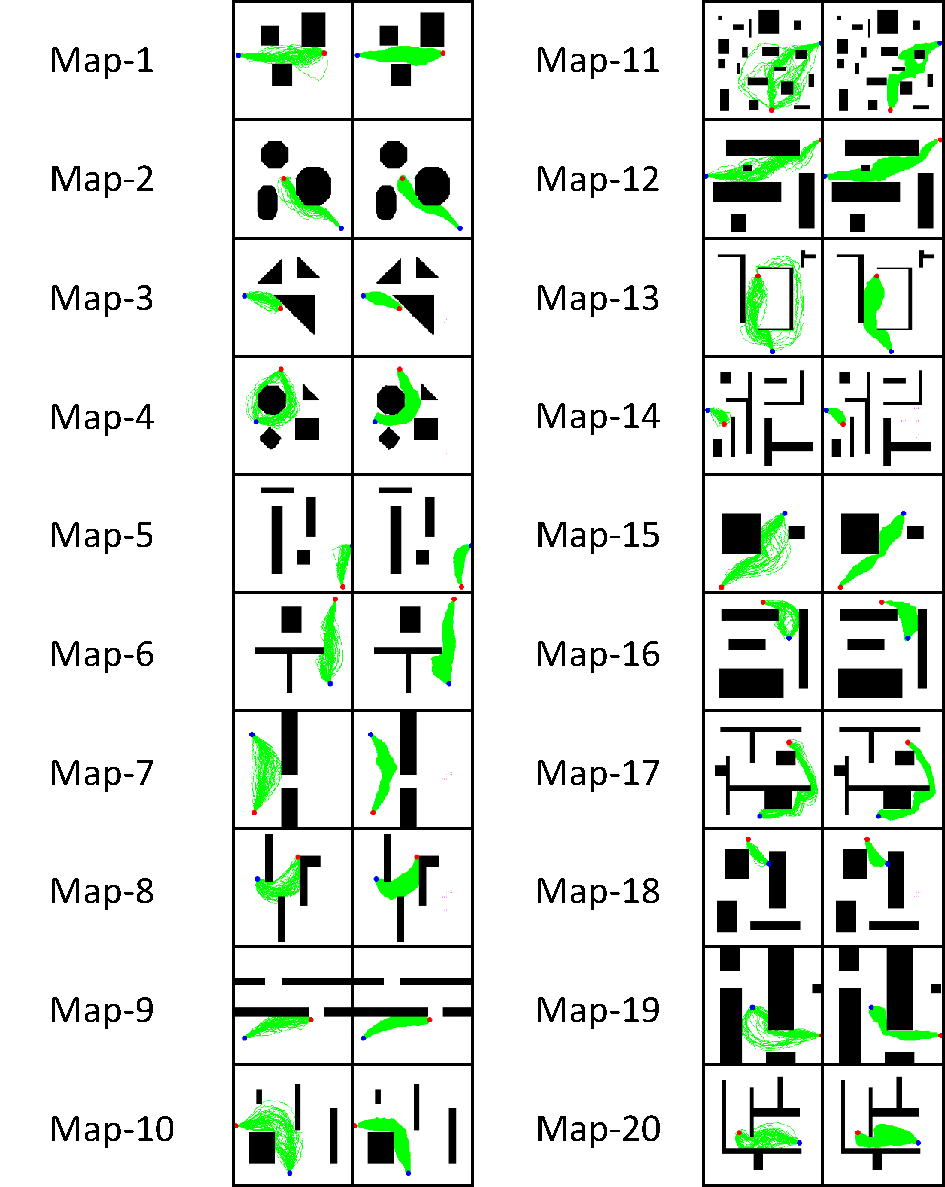
\includegraphics[width=1\linewidth]{generate-data-comparsion.pdf}
	\caption{Demonstration of model generation effects.
	On the left is the map name.
	The first column is the ground truth.
	The second column is the promising regions generated by the model.
	The black parts are obstacles.
	The blue dot is the starting point and the red dot is the end point.
	Green areas are promising areas.
	}     
	\label{fig: generate-data-comparsion}
\end{figure}

Fig. \ref{fig: generate-data-comparsion} demonstrates the promising regions for model generation.
The leftmost of each column is the map name, and the middle is the ground truth.
On the far right is a promising region for model generation.
In each image, black dots represent obstacles, blue dots represent starting points, and red dots represent end points.
It is worth noting that the promising regions generated by the model are tighter than the ground truth.

\subsection{Comparison with RRT*}
As a path planning problem, we employ three main metrics to evaluate the performance of the algorithm.
The main indicators include path cost, number of nodes, and time-consuming.
We will conduct multiple experiments on different maps to demonstrate the superiority of our algorithm.

First, we compare the resources consumed by a single iteration.

Fig. \ref{fig: ours on map1} and Fig. \ref{fig: rrt-star on map1} show the iterative process of our algorithm and RRT* to obtain the initial path on Map-1, and the green area indicates the promising area.
Red lines represent explored regions, dark blue lines represent initial paths.
The initial path cost obtained by CGRRT* is 215.94, the consumption time is 0.00052s, and the total number of nodes is 246.
The initial path cost obtained by RT* is 234.11, the consumption time is 0.00014s, and the total number of nodes is 113.

It can be seen that in terms of path quality, the path quality generated by our algorithm is better.
In terms of resource consumption to obtain the initial path, our algorithm requires less resources and has faster convergence speed.
\begin{figure}[htbp]
	\centering
	\begin{minipage}[t]{0.45\textwidth}
		\centering
		\includegraphics[width=\textwidth]{our-init-path.eps}
		\caption{Ours, Cost = 215.94, Time = 0.00052s, Nodes = 246.}
		\label{fig: ours on map1}
	\end{minipage}
	\begin{minipage}[t]{0.45\textwidth}
		\centering
		\includegraphics[width=\textwidth]{rrt-init-path.eps}
		\caption{RRT*, Cost=234.11, Time=0.00014, Nodes=113.}
		\label{fig: rrt-star on map1}
	\end{minipage}
\end{figure}

\subsection{Comparison experiments}
In this section, we conduct repeated experiments comparing our algorithm with the most popular algorithm (RRT*).

% 11 13 17 19 20
\begin{table}[ht]
	\centering
	\begin{tabular}{l|c|c|c|c|c}
	\toprule
	\multirow{2}{*}{Algorithm} & \multicolumn{5}{c}{Maps} \\
	\cline{2-6}
	& Map 11 & Map 13 & Map 17 & Map 19 & Map 20 \\
	\midrule
	Ours & 233.7 $\pm$ 11.5 & 202.4 $\pm$ 7.0 & 294.6 $\pm$ 9.5 & 208.7 $\pm$ 7.2 & 159.3 $\pm$ 9.2 \\
	\midrule
	RRT* & 271.1 $\pm$ 33.1 & 244.2 $\pm$ 38.9 & 319.3 $\pm$ 20.2 & 253.4 $\pm$ 25.7 & 192.9 $\pm$ 25.3 \\
	\bottomrule
	\end{tabular}
	\caption{Comparison of path costs on different maps.}
	\label{tab: costs}
\end{table}

\begin{table}[ht]
	\centering
	\begin{tabular}{l|c|c|c|c|c}
	\toprule
	\multirow{2}{*}{Algorithm} & \multicolumn{5}{c}{Maps} \\
	\cline{2-6}
	& Map 11 & Map 13 & Map 17 & Map 19 & Map 20 \\
	\midrule
	Ours & 285 $\pm$ 71 & 168 $\pm$ 70 & 311 $\pm$ 54 & 295 $\pm$ 75 & 151 $\pm$ 44 \\
	\midrule
	RRT* & 896 $\pm$ 645 & 1215 $\pm$ 993 & 739 $\pm$ 597 & 1729 $\pm$ 824 & 603 $\pm$ 521 \\
	\bottomrule
	\end{tabular}
	\caption{Comparison of the number of nodes to obtain the initial path on different maps.}
	\label{tab: nodes}
\end{table}

\begin{figure}
	\centering
	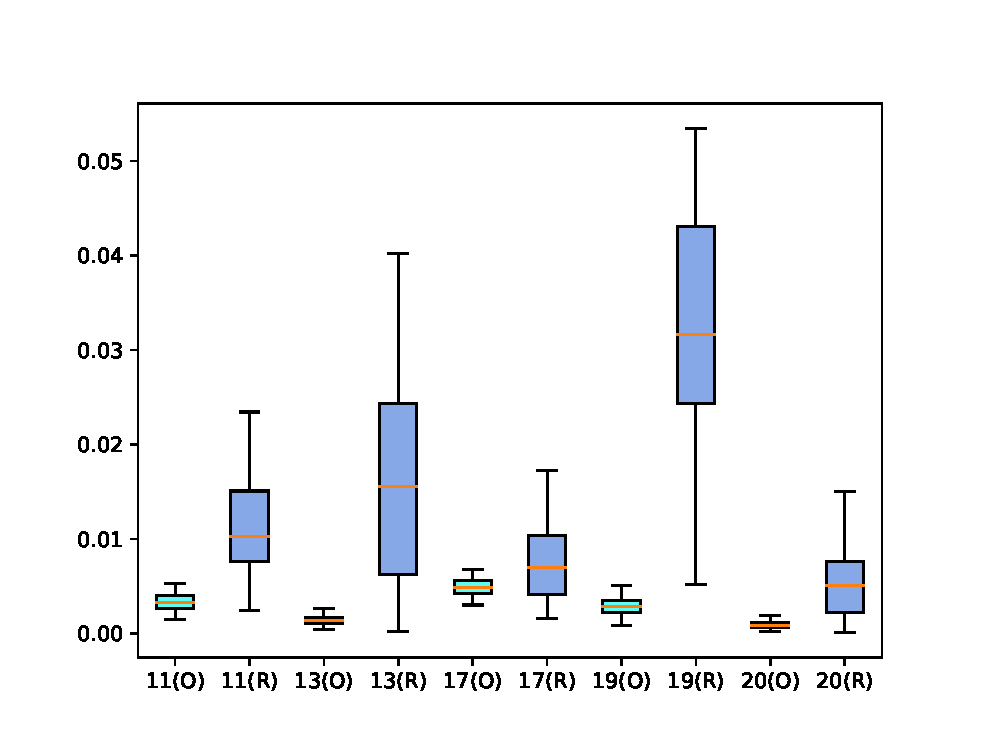
\includegraphics[width=1\linewidth]{first_time.eps}
	\caption{Comparison of the time taken to obtain the initial path on different maps.
	The x-axis is a different map, and the brackets indicate different algorithms.
	O denotes our algorithm and R denotes RRT*.
	The y-axis represents the elapsed time in seconds.}
	\label{fig: time}
\end{figure}


\subsection{Discussion}


\section{Conclusion and further work}\label{section: conclusions}
In this paper, we propose a learning-based path planning algorithm.
First, we use GAN to learn the planner from the data of successful plans.
Second, use the planner to give promising areas to the map that needs to be planned.
Finally, RRT* is used for path planning in promising areas to generate the final path.

For the algorithm proposed in this paper, we designed twenty different original maps.
The original map has been expanded to 200 enhanced maps.
Each map consists of 50 pairs of random starting and ending points and planned trajectories to form a data set of 10,000 pieces.

Eighty percent of the 10,000 data sets are used for training, and the remaining 20 percent are used for testing model performance.

Finally, we compared different indicators with the two most popular algorithms at the moment.
Experimental results demonstrate that our algorithm achieves a convincing lead in terms of generated promising regions, path quality, and efficiency.
Our future work mainly includes the following aspects:
\begin{enumerate}
	\item Collect real-world trajectory data and build a GAN model that is suitable for training and available in reality.
	\item Add dynamical constraints to fit the generated promising regions and the resulting trajectories sociologically.
\end{enumerate}

\begin{acknowledgements}
This work was supported by the National Social Science Foundation of China under Grant No. 22FZXB092.

\end{acknowledgements}

\section*{Data availability statement}
Data will be available upon reasonable request.

\bibliographystyle{splncs}

\bibliography{main}

\end{document}
